%%% Chasopys Krayany
%%% ---------------
%%% PREAMBLE
%%% ---------------
\documentclass[10pt,a4paper]{article}

% Define geometry (without using the geometry package)
\setlength\topmargin{-48pt}
\setlength\headheight{20pt}
\setlength\headsep{0pt}
\setlength\marginparwidth{-20pt}
\setlength\textwidth{7.0in}
\setlength\textheight{10.0in}
\setlength\oddsidemargin{-30pt}
\setlength\evensidemargin{-30pt}

\frenchspacing						% better looking spacing

% Call packages we'll need
\usepackage[utf8]{inputenc}
\usepackage{CJKutf8}
\newenvironment{Japanese}{%
  \CJKfamily{min}%
  \CJKtilde
  \CJKnospace}{}
\usepackage[english,ukrainian]{babel}			% languages
\usepackage{graphicx}				% images
\usepackage{amssymb,amsmath}		% math
\usepackage{multicol}				% three-column layout
\usepackage{url}					% clickable links
\usepackage{marvosym}				% symbols
\usepackage{wrapfig}				% wrapping text around figures
\usepackage[T1,T2A]{fontenc}			% font encoding
\usepackage{charter} 				% Charter font for main content
\usepackage{blindtext}				% dummy text
\usepackage{datetime}				% custom date
	\newdateformat{mydate}{\monthname[\THEMONTH] \THEYEAR}
\usepackage[pdfpagemode=FullScreen,
			colorlinks=false]{hyperref}	% links and pdf behaviour

\makeatletter\chardef\l@japanese=255 \makeatother

% Customize (header and) footer
\usepackage{fancyhdr}
\pagestyle{fancy}
\lfoot{	\footnotesize 
Спільнота українців Японії ''Краяни'' / 
\begin{CJK}{UTF8}{}
\begin{Japanese}
在日ウクライナ人コミュニティ「クラヤニイ」
\end{Japanese}
\end{CJK}
\\
		\Mundus\ \href{https://www.facebook.com/ukrainians.japan}{www.facebook.com/ukrainians.japan}	\quad
	  }
\cfoot{}
\rfoot{\footnotesize ~\\ Сторінка \thepage}
\renewcommand{\headrulewidth}{0.0pt}	% no bar on top of page
\renewcommand{\footrulewidth}{0.4pt}	% bar on bottom of page

%%% ---------------
%%% DEFINITIONS
%%% ---------------

% Define separators
\newcommand{\HorRule}[1]{\noindent\rule{\linewidth}{#1}} % Creating a horizontal rule
\newcommand{\SepRule}{\noindent							 % Creating a separator
						\begin{center}
							\rule{250pt}{1pt}
						\end{center}
						}						

% Define Title en News input
\newcommand{\JournalName}[1]{%
		\begin{center}	
			\Huge \usefont{T2A}{augie}{m}{n}
			#1%
		\end{center}	
		\par \normalsize \normalfont}
		
\newcommand{\JournalIssue}[1]{%
		\hfill \textsc{\mydate \today, Випуск №1}
		\par \normalsize \normalfont}

\newcommand{\NewsItem}[1]{%
		\usefont{T2A}{iwona}{m}{n} 
		\large #1 \vspace{4pt}
		\par \normalsize \normalfont}
		
\newcommand{\NewsAuthor}[1]{%
			\hfill \textsc{#1} \vspace{4pt}
			\par \normalfont}		


%%% ---------------
%%% BEGIN DOCUMENT
%%% ---------------
\begin{document}
% Title	
% -----
\JournalIssue{1}
		\includegraphics[width=1\textwidth]{../common_files/chasopys_logo}
%\JournalName{Краяни - часопис українців Японії}
\noindent\HorRule{3pt} \\[-0.75\baselineskip]
\HorRule{1pt}
% -----

% Front article
\vspace{0.5cm}
	\SepRule
\vspace{0.1cm}

\begin{center}
\begin{minipage}[h]{0.75\linewidth}
	\begin{wrapfigure}{l}{0.61\textwidth}
		\includegraphics[width=0.62\textwidth]{images/bunkamura}
		\\	% this spacer is needed to make the text on the right fit OK
	\end{wrapfigure}
	\NewsItem{Писанки в Шібуя}
Виставка робіт українських та японських майстринь писанкарства була представлена на щорічній виставці ''Bunkamura Craft Collection 2015'', що в районі Шібуя Токіо.
\vspace{3.3cm}
\end{minipage}
\end{center}

% Page 1
\vspace{0.5cm}
	\SepRule
\vspace{0.5cm}
\begin{multicols}{3}
	\NewsItem{Вітаємо з перемогою!}
	\NewsAuthor{Москва}
		\begin{center}
			\includegraphics[width=0.8\linewidth]{images/rapiry}
		\end{center}
Вітаємо Олега Мацейчука - українця, головного тренера з фехтування на рапірах Японії, з перемогою вихованця, чемпіона світу з фехтування Юкі Ота (Японія). 
У фіналі чемпіонату світу серед чоловіків у двобої з американцем переміг японець. Золото з фехтування на рапірах стало першим в історії Японії.
Олег Мацейчук - киянин, екс-фехтувальник збірної України. В 2003 розпочав роботу тренером з фехтування в Японії. За період перебування в Японії виховав ціле покоління спортсменів, які вже самі стали тренерами.
Успіхів та нових досягнень!

\vspace{1cm}
\NewsItem{Цікаві семінари в Кансай}
\NewsAuthor{Кіото}
		\begin{center}
			\includegraphics[width=0.8\linewidth]{images/seminary}
		\end{center}
Запрошуємо усіх, хто цікавиться українською культурою, відвідати ''Цікаві семінари'', що організує спільнота українців у Кансаї. На семінарах ми розкажемо про основні поточні події у житті спільноти, познайомимо з історією, мистецтвом і культурою нашої країни. Семінари відбудуться 11-го і 25-го липня (субота) з 15:00 до 16:30 у кокока (Міжнародному Центрі міста Кіото). Участь у семінарах платна: 1,000 ієн за участь у 2-х семінарах. Кошти від семінару підуть на розвиток української громади. Також будемо збирати пожертви для постраждалих у війні на сході. Ми готуємо багато цікавих презентацій. Учасники семінарів зможуть вдягнути український костюм, а також скуштувати українських солодощів. Семінари будуть проходити японською мовою. 
\end{multicols}

\newpage

% Page 2
\begin{multicols}{3}

	\NewsItem{Благодійний концерт}
	\NewsAuthor{Йокогама}
		\begin{center}
			\includegraphics[width=0.8\linewidth]{images/concert}
		\end{center}
20 червня в м. Йокогама відбувся благодійний концерт на підтримку Військового Госпіталю України ''Charity For Ukraine, 2015''.
Чудовий концерт організували талановиті артисти та виконавці різних країн: Elina-star, Kateryna, Yuliya, Viktoria, Amauri Marina, Cesar Canisales, Lana, Itsuki, Erina, Emma, Eshe, Anzy, Hikari, Leila, Yasmin. Захід відбувся за підтримки Посольства України в Японії.

\vspace{1cm}
\NewsItem{''Івасик Телесик'' в Японії}
\NewsAuthor{Токіо, школа ''Джерельце''}
		\begin{center}
			\includegraphics[width=0.8\linewidth]{images/telesyk}
		\end{center}
''Івасик Телесик'' в Токio на останньому уроці недільної школи Джерельце 14 червня. В День ''останнього дзвоника'' японського Джерельця вихованці школи порадували батьків та вчителів виставою, за казкою ''Івасик Телесик''. За успіхи у навчанні учні отримали вітальні грамоти та подарунки. Українська дитяча школа ''Джерельце'' була заснована у березні 2009 року в місті Токіо. Заняття в школі проводяться двічі на місяць кваліфікованими вчителями за власно розробленою програмою. Сьогодні кількість вихованців нараховує більше 40 учнів різних вікових категорій. Дітлахи мають змогу навчитись читанню, письму, математиці та мистецтву. Діти знайомляться з традиційними святами, готують Новорічні та Великодні вистави, Різдвяні Вертепи. Отримати більше інформації та записатись на заняття можна на сайті школи dzherelce.github.io 

\vspace{1cm}
	\NewsItem{3-й щорічний Мегамарш у вишиванках}
	\NewsAuthor{Токіо, Ґінза}
		\begin{center}
			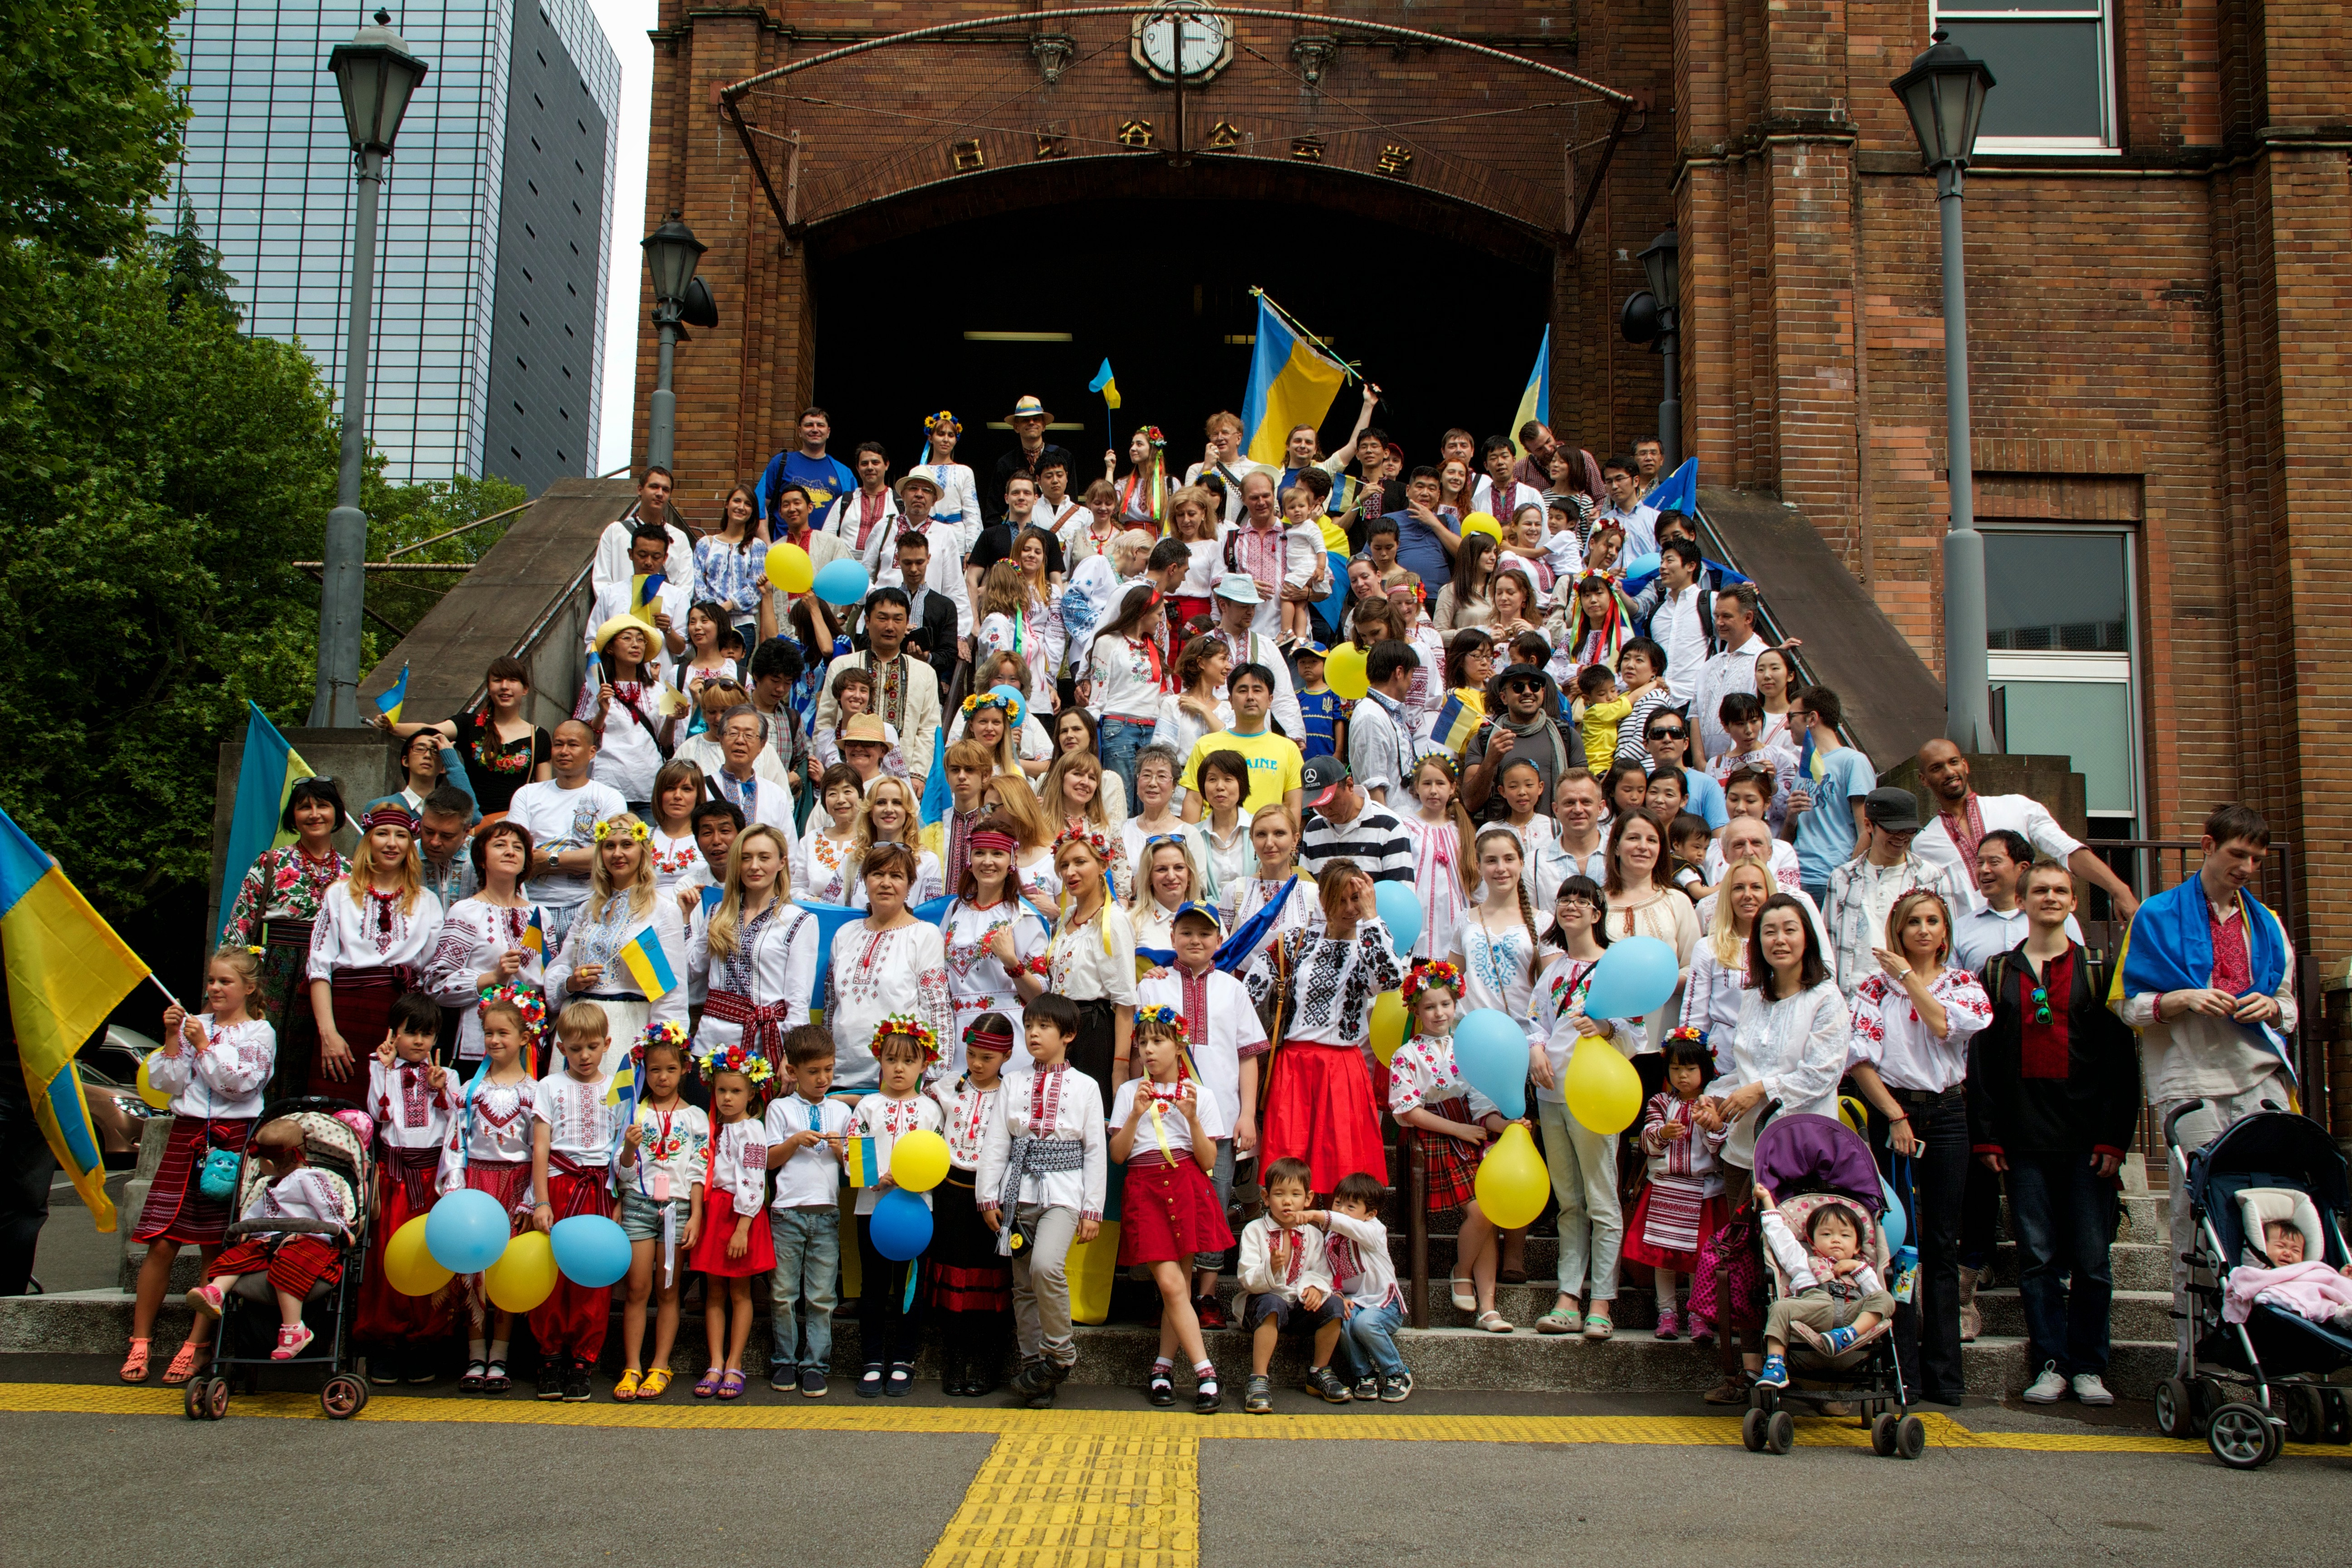
\includegraphics[width=0.8\linewidth]{images/megamarsh}
		\end{center}
Дякуємо всім, хто взяв участь у 3-му щорічному Мегамарші у вишиванках у Токіо! Більше 150 українців, японців та представників інших країн світу вийшли у вишитих сорочках та з прапорами України, викликавши неабиякий інтерес у місцевого населення. Захід був організований за підтримки Посольства України в Японії та місії Української Православної Церкви Київського Патріархату ''St. Jude Ukrainian Orthodox Mission'' в місті Токіо. Цьогорічний парад був присвячений співпраці між Україною та Японією. Прапор України, що побував на Майдані у Києві, до Токіо привезла студентка з Калуша, об'єднавши українців Японії з Батьківщиною. Захід підтримав дипломатичний сектор Посольства України в Японії і надзвичайний і повноважний Посол Ігор Харченко з сім'єю. У вишиванках приєднались екс-посол Японії в Україні Саката Тоїчі з дружиною, а також відомий українознавець та генерал-полковник Українського Реєстрового Козацтва Йошіхіко Окабе. Вишиванкова хода в Токіо стала гарною традицією, а постійно зростаюча чисельність учасників та активний інтерес японців до заходу підтвердили необхідність гуртування та створення українського осередку в Японії. Слава Україні!

\vspace{1cm}
\NewsItem{Токійський Козак}
\NewsAuthor{Токіо}
		\begin{center}
			\includegraphics[width=0.8\linewidth]{images/kozak}
		\end{center}
Обирай українське, де б ти не був! Японці вражають своєю любов'ю до України та українського. Їдучи у справах по дорозі в Токіо українка почула сигнал іншого авто. Спочатку подумала, що вона порушила правила і за це їй сигналять. Її обганяє японець і з щасливою японською посмішкою вказує на свою машину, де наклейки з написом ''Україна'' та ''Козак'' та на її, де зображений український прапор. Так знаходять нових друзів по авто. Користуйтесь транспортними послугами ''Козака''! 

\vspace{1cm}
\NewsItem{Миру Україні!}
\NewsAuthor{Танабата 2015}
		\begin{center}
			\includegraphics[width=0.8\linewidth]{images/tanabata}
		\end{center}
Побажання українців Японії на фестивалі Танабата. Японці вірять, що якщо 7-го липня написати своє бажання, то воно обов'язково здійсниться!

\end{multicols}

\newpage

% Page 3
\begin{multicols}{3}

\NewsItem{Йван Канеда - диякон української церкви}
\NewsAuthor{Токіо}
		\begin{center}
			\includegraphics[width=0.8\linewidth]{images/kaneda}
		\end{center}
Разом з українською громадою в Японії, розвивається і українська православна церква в Токіо. Так, на вересень 2015 року заплановано висвячення в диякона місії Української Православної Церкви Київського Патріархату в Японії Йвана Канеди. Дасть Бог, Йван стане першим священиком-японцем нашої церкви.

\vspace{2cm}
\NewsItem{Українське мистецтво в Японії}
\NewsAuthor{Фуджіока}
		\begin{center}
			\includegraphics[width=0.8\linewidth]{images/mischak}
		\end{center}
Перша виставка картин українського митця в Японії Андрія Міщака відкрилась у місті Фуджіока, префектура Ґунма.

\vspace{1cm}
\NewsItem{Концерт пам'яті жертв трагедії на АЕС Фукушіма}
\NewsAuthor{Кіото}
		\begin{center}
			\includegraphics[width=0.8\linewidth]{images/concert-fukushima}
		\end{center}
В 4-ту річницю трагедії на АЕС Фукушіма-1 в місті Кіото звучала українська бандура. 11 березня там відбувся захід, присвячений пам'яті загиблих та постраждалих внаслідок аварії на АЕС Фукушіма-1. Бандуристка Наталя Ґудзій виступила з українськими мелодіями та піснями, а також розповіла про загублені домівки українців після аварії на Чорнобильській АЕС.

\vspace{1cm}
\NewsItem{Христос Воскрес!}
\NewsAuthor{Великдень 2015}
		\begin{center}
			\includegraphics[width=0.8\linewidth]{images/paska}
		\end{center}
Українська громада Японії відсвяткувала Великдень в українській церкві в Токіо, після чого був організований святковий пікнік у колі друзів.
\end{multicols}

\newpage

% Page 4
\begin{multicols}{3}
\NewsItem{Майстер-клас з української кухні}
\NewsAuthor{Акаші, Хьоґо}
		\begin{center}
			\includegraphics[width=0.8\linewidth]{images/ukr-cuisine-akashi}
		\end{center}
В місті Акаші, префектура Хьоґо, 4 березня відбувся майстер клас з приготування українських страв. За ініціативи Міжнародної асоціації міста Акаші Ольга Балинська та ще 20 містян зібрались на український обід. Навчались готувати український борщ, млинці з грибами та яблуками та салат з крабовими паличками. По обіді гостя заходу розповіла про Україну, кухню та вишиванки. Всім японським учасникам борщ та страви були до смаку і вони вже чекають наступного разу!

\vspace{1cm}
\NewsItem{Український вечір}
\NewsAuthor{Канаґава}
		\begin{center}
			\includegraphics[width=0.8\linewidth]{images/ukr-evening}
		\end{center}
Вдруге в Японії, 22 лютого, в залі ГО ''Японія-країни Євразії'' у префектурі Канаґава відбувся ''Український вечір'' в рамках якого була виконана моновистава ''Княжна'' (за поемами Т.Г.Шевченка ''Відьма'', ''Княжна'') у виконанні Наталі Морозової-Шімади, переклад Оксани Піскунової, а також презентація України, її культури та звичаїв Оксаною Свистак.

Всіх присутніх вітала виставка старовинних українських книг, предметів побуту, вишиванок та рушників. Оксана Свистак розпочала вечір презентацією про Україну. Вихованка української школи в Токіо ''Джерельце'' Юлія привітала всіх присутніх чарівною піснею. У продовження вечора на всіх чекала вистава ''Княжна''. Наталя Морозова-Шімада виконувала виставу українською мовою, однак на екрані слова акторки дублювались японським перекладом, даючи змогу всім присутнім відчути силу Шевченкового слова.

Захід відвідали багато японців, кому цікава та небайдужа Україна, її культура та звичаї: студенти, працівники компаній, дослідники, духовенство. Під час прес-конференції присутні гості та представники ЗМІ задавали питання про українські вареники, жанр спектаклю, ситуацію в Україні, відомих українців та цікавились наступними подіями пов'язаними з Україною в Японії.

Фото: Юрій Свистак, Katsutaro Alexy Hirayama, Naoya Sakurai
\end{multicols}

\newpage

% Page 5
\begin{multicols}{3}
\NewsItem{Ласкаво просимо до ''Джерельця''!}
\NewsAuthor{Токіо}
		\begin{center}
			\includegraphics[width=0.8\linewidth]{images/dzherelce}
		\end{center}
Українська школа для дітей "Джерельце" в Токіо запрошує дітлахів на навчання! Подробиці щодо діяльності школи, розкладу занять та інша інформація - на сайті http://dzherelce.github.io/
Українська школа для дітей розпочала свою роботу у березні 2009 року. Головною метою школи є навчити дітей українських та багатонаціональних родин розуміти та спілкуватись українською мовою, познайомити з дитячим фольклором, українською культурою, підтримувати та зберігати традиції свого народу. Професійні вчителі навчають малят читанню, письму, математиці, мистецтву. Разом з батьками і вчителями вихованці знайомляться з традиціями Батьківщини, готують новорічні та Великодні вистави, Різдвяні вертепи, навчаються розписувати писанки на Великдень. Вихідні проводять в захоплюючих походах у гори або у літньому таборі. Майбутнє України народжується тут!

\vspace{1cm}
\NewsItem{Акція-протест проти російської агресії на Донбасі та в Криму}
\NewsAuthor{Токіо}
		\begin{center}
			\includegraphics[width=0.8\linewidth]{images/protest}
		\end{center}
18 січня 2015 року українці Японії приєдналися до всесвітньої акції миру та солідарності із загиблими громадянами неподалік міста Волноваха. Захід відбувся біля посольства Російської Федерації в м. Токіо.
Учасники виголосили вимогу негайного припинення агресії проти України та анексії АР Крим, а також звільнення Савченко Н.В., Сенцова О.Г., інших викрадених та незаконно ув’язнених громадян України. Викладені у письмовій формі вимоги, підписані усіма присутніми учасниками акції, активісти у супроводі поліцейських віднесли до посольства Росії. Проте, як і раніше, змушені були опустити петицію у поштову скриньку. Зі сторони російської амбасади українці не отримали жодної відповіді.
Для японських ЗМІ та громадськості активісти нагадали про військові дії в Україні та смерті мирних людей, що продовжуються до сьогодні. Учасники акції нагадали про українських політичних в’язнів і голодування Савченко Н.В.
В пам’ять загиблих українських громадян, захисників України та жертв репресій учасники акції заспівали пісню «Пливе кача».
Спільно зі священником місії УПЦ КП St. Jude Ukrainian Orthodox Mission, Tokyo учасники помолились за народ України, Боже благословення та мирне врегулювання конфлікту, завершили акцію виконанням гімну України.

\vspace{1cm}
\NewsItem{Мир і війна очима дітей}
\NewsAuthor{Кіото}
		\begin{center}
			\includegraphics[width=0.8\linewidth]{images/war-and-peace}
		\end{center}
Мир і війна очима дітей - благодійна виставка робіт вихованців шкіл Донецької області з міст Слов'янськ та Краматорськ відбулась 10-11 січня у Міжнародному центрі міста Кіото.
Насичені яскравими барвами, теплом та любов'ю, дітлахи українських шкіл зобразили їхні мрії та бажання, бачення та сподівання. Багато робіт містило блакитні та жовті кольори, українську символіку, часто зображали родину, птахів та звірів, сонце, школу, мирне життя. Не зважаючи на те, якою мовою були підписані роботи: українською чи російською, з малюнків віяло теплом та сподіваннями на те, що якнайскорше відновиться мир і в Україні все буде добре.
Всім відвідувачам організатори розказали про події в Україні, про життя дітей у зоні бойових дій, демонстрували знімки учнів, відео записи їх мистецьких творів. 
Під час заходу проводився збір коштів на купівлю теплого одягу, повсякденних речей для дітей. Деякі з відвідувачів приносили теплі речі і просили їх передати в Україну.
Захід відбувся за ініціативи київського видавництва та за підтримки представника Президента України в Донецькій та Луганській області з української сторони, та за підтримки ''Товариства дружби Кіото і Києва'' та балетної школи міста Кіото - з японської. Всього було зібрано більше 700 дитячих робіт на тему ''Мир і війна очима дітей''! У виставковому центрі в Кіото в аудиторії були презентовані тільки 100 робіт учнів 16 шкіл та інтернатів Донбасу, які зобразили своє бачення миру та війни. Інша частина робіт буде представлена в Українському домі в Китаї, Великобританії та США.

\end{multicols}

\end{document} 

